\documentclass[twoside,12pt]{article}
\usepackage{amsmath,amsfonts,amsthm,fullpage,amssymb}
\usepackage{algorithm,hyperref}
\usepackage{algorithmic}
\usepackage{graphicx}
\usepackage{tcolorbox}


\begin{document}

\title{ISYE 6740, Fall 2020, Homework 2\\ {\small 100 points + 15 bonus points}}
\author{Prof. Yao Xie}
\date{}
\maketitle

\subsection*{1. PCA: Food consumption in European countries [50 points]}

The data \textsf{food-consumption.csv} contains 16 countries in Europe and their consumption for 20 food items, such as tea, jam, coffee, yogurt, and others. We will perform principal component analysis to explore the data. In this question, please implement PCA by writing your own code (you can use any basic packages, such as numerical linear algebra, reading data, in your file).


\vspace{.1in}
First, we will perform PCA analysis on the data by treating each country's food consumption as their ``feature'' vectors. In other words, we will find weight vectors to combine 20 food-item consumptions for each country.  
 
\begin{enumerate}

\item (10 points) For this problem of performing PCA on countries by treating each country's food consumption as their ``feature'' vectors, explain how the data matrix is set-up in this case (e.g., the columns and the rows of the matrix correspond to what). 
\begin{tcolorbox}
\textbf{Solution:} Each row corresponds to a country and each component in this row represents the food consumption of this country on a particular food-item. Each column corresponds to a food-item and each component in this column represents the consumption of this food in a particular country.
\end{tcolorbox}

\item (10 points) Suppose we aim to find top $k$ principal components. Write down the mathematical optimization problem for solving this problem (i.e., PCA optimization problem). Show why the first principal component is obtained by using a weight vector corresponding to the eigenvectors associated with the largest eigenvalue. Explain how to find the rest of the principal components. 
\begin{tcolorbox}
\textbf{Solution:} Suppose we have $m$ data points $x^1, x^2, ..., x^m \in R^n$, with their mean $\mu = \frac 1 m \sum_{i=1}^m x^i$. The mathematical optimization problem for finding top $k$ principle components is to find $k$ orthogonal directions $w^1, w^2, ..., w^k \in R^n$ where $\|w^j\| \leq 1$ for $j = 1, 2, ..., k$, such that the variance of the data along those directions is maximized, i.e. find
$$\max_{w^1, w^2, ..., w^k} \frac 1 m \sum_{j=1}^{k} \sum_{i=1}^m ((w^j)^T(x^i-\mu))^2,$$ which can be simplified to $$\max_{w^1, w^2, ..., w^k}  \sum_{j=1}^{k} (w^j)^TCw^j,$$ with constraints 
$$\|w^j\| \leq 1 \text{ and } w^i \perp w^j \text{ if } i \neq j \text{ for } i, j = 1, 2, ..., k.$$ Here $C = \frac 1 m \sum_{i=1}^m (x^i - \mu)(x^i-\mu)^T$ is the covariance matrix. 
To solve this optimization problem, we apply the method of Lagrange multipliers with multiple constraints, which transform the optimization problem into solving the following equations $$\sum_{j=1}^k Cw^j - \sum_{j=1}^k \lambda_jw^j = \sum_{j=1}^k (Cw^j - \lambda_jw^j) = 0.$$Since $w^1, w^2, ..., w^k$ are orthogonal with each other, the equation above is equivalent to $$Cw^j = \lambda_j w^j, \quad j = 1, 2, ..., k.$$ So the problem becomes finding $$\max_{w^1, w^2, ..., w^k}  \sum_{j=1}^{k} \lambda_j \|w^j\|^2,$$
with constraints $$\|w^j\| \leq 1, \quad j = 1, 2, ..., k.$$ 
Therefore, we just need to find the $k$ largest eigenvalues and the corresponding eigenvectors of $C$ to solve the optimization problem. When $k = 1$, the first principal component can be obtained by finding the eigenvector $w^1$ of $C$ corresponding to the largest eigenvalue. To find the rest of the principle components, we can apply eigen-decomposition to $C$, i.e. $C = U\Lambda U^T$. Alternatively, we can directly apply SVD to the normalized data matrix $X = [x^1-\mu, x^2-\mu, ..., x^m - \mu] = U\Sigma V^T$. In both methods, the first $k$ column vectors $w^1, w^2, ..., w^k$ will be the $k$ eigenvectors of $C$ corresponding to the largest $k$ eigenvalues. 
\end{tcolorbox}

\begin{tcolorbox}
To find the $k$ principal components of a data point $x^i$, we just need to compute 
$$ z^i = \left( \begin{array}{c} (w^1)^T(xi-\mu)/\sqrt{\lambda_1} \\ (w^2)^T(xi-\mu)/\sqrt{\lambda_2} \\ ...\\ (w^k)^T(xi-\mu)/\sqrt{\lambda_k} \end{array} \right).$$
\end{tcolorbox}

\item (10 points) Now assume $k = 2$, i.e., we will find the first two principal components for each data point. Find the weight vectors $w_1$ and $w_2$ to extract these two principal components. Plot these two weight vectors, respectively (e.g., in MATLAB, you can use \textsf{stem(w)} to plot the entries of a vector $w$; similar things can be done in Python). Explain if you find any interesting patterns in the weight vectors. 
\begin{tcolorbox}
\textbf{Solution:} Below are the plots of the two weight vectors $w_1$ and $w_2$. As we can see, both $w_1$ and $w_2$ have some zero components. But their zero components do not overlap, meaning that they are emphasizing on different features. \\
 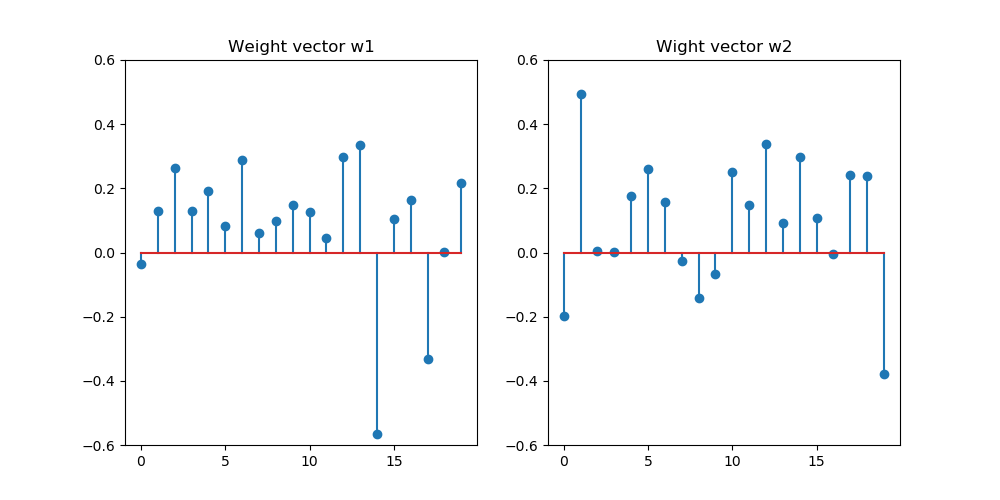
\includegraphics[width=.99\textwidth]{weights_vectors.png}
\end{tcolorbox}

\item (10 points) Now extract the first two principal components for each data point (thus, this means we will represent each data point using a two-dimensional vector). Draw a scatter plot of two-dimensional representations of the countries using their two principal components. Mark the countries on the lot (you can do this by hand if you want). Please explain any pattern you observe in the scatter plot.
\begin{tcolorbox}
\textbf{Solution:} There are some interesting patterns in the following scatter plot. The data points are naturally scattered out and do not overlap with each other, showing that our principal components are doing a good job in representing the variances of the data. Moreover, some countries that are geographically close to each other are also close to each other in the scatter plot, like Finland, Sweden, Norway and Denmark. This makes sense because usually people living in the same area tend to have similar eating habits. In conclusion, the result shows that PCA is a very useful tool to reduce the dimension of our data so that we can properly visualize the data in a plane and preserve the relationship between data points at the same time.\\ 
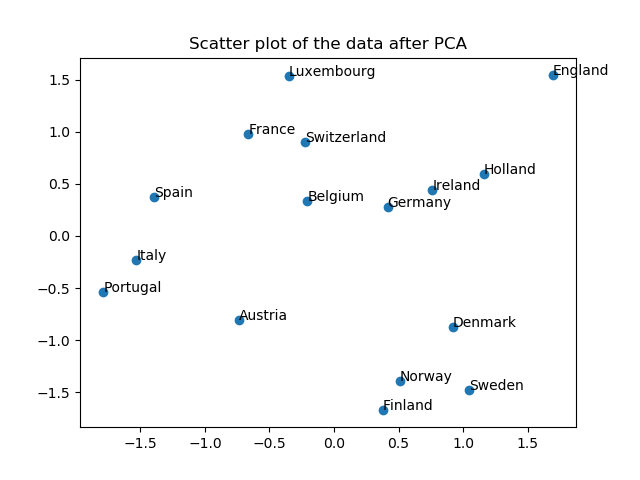
\includegraphics[width=.99\textwidth]{scatter1.png}
\end{tcolorbox}

\end{enumerate}

Now, we will perform PCA analysis on the data by treating country consumptions as ``feature'' vectors for each food item. In other words, we will now find weight vectors to combine country consumptions for each food item to perform PCA another way.
\begin{enumerate}
\item[5. ] (10 points) Project data to obtain their two principle components (thus, again each data point -- for each food item -- can be represented using a two-dimensional vector). Draw a scatter plot of food items. Mark the food items on the plot (you can do this by hand if you do not want). Please explain any pattern you observe in the scatter plot.
\begin{tcolorbox}
\textbf{Solution:} From the scatter plot we see that some similar items are close to each other. For example, apples and oranges, butter and margarine, as well as frozen fish and frozen veggies.  This makes sense because if the people in a country like to buy one kind of food, they will buy several similar food items. For instance, if the people in some country like to buy frozen foods, then they will consume a lot of frozen fish and frozen veggies. But if they think frozen food is not healthy, they will consume very little frozen food, including both frozen fish and frozen veggies. 
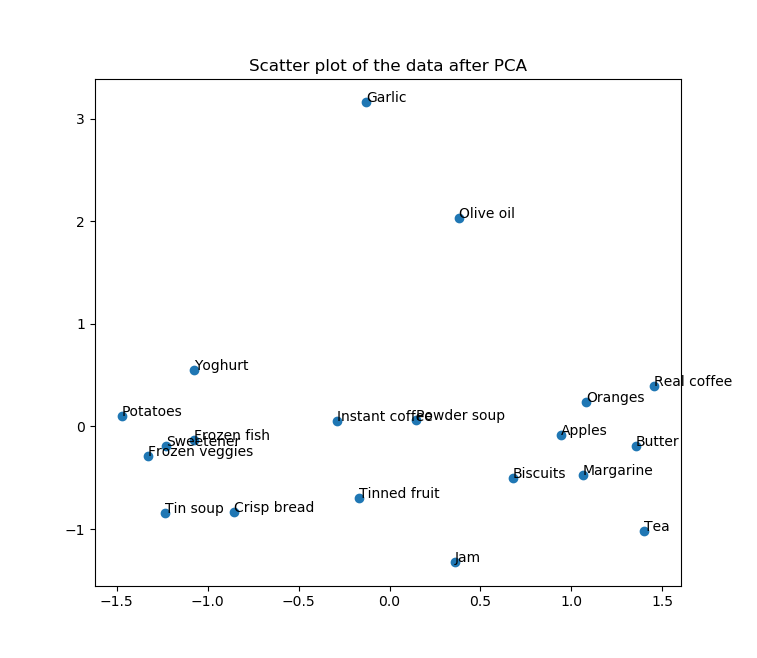
\includegraphics[width=.99\textwidth]{scatter2.png}
\end{tcolorbox}
\end{enumerate}


%\clearpage

\subsection*{2. Order of faces using ISOMAP [50 points]}

This question aims to reproduce the ISOMAP algorithm results in the original paper for ISOMAP, J.B. Tenenbaum, V. de Silva, and J.C. Langford, Science 290 (2000) 2319-2323 that we have also seen in the lecture as an exercise (isn't this exciting to go through the process of generating results for a high-impact research paper!) 


The file \textsf{isomap.mat} (or \textsf{isomap.dat}) contains 698 images, corresponding to different poses of the same face. Each image is given as a 64 $\times$ 64 luminosity map, hence represented as a vector in $\mathbb R^{4096}$. This vector is stored as a row in the file. [This is one of the datasets used in the original paper] In this question, you are expected to implement the ISOMAP algorithm by coding it up yourself. You may use the provided functions in \textsf{ShortestPath.zip} to find the shortest path as required by one step of the algorithm. 

Choose the Euclidean distance (i.e., in this case, a distance in $\mathbb R^{4096}$) to construct the nearest neighbor graph—vertices corresponding to the images. Construct a similarity graph with vertices corresponding to the images, and tune the threshold $\epsilon$ so that each node has {\it at least} 100 neighbors (this approach corresponds to the so-called $\epsilon$-Isomap).

\begin{enumerate} 

\item[(a)] (10 points) Visualize the similarity graph (you can either show the adjacency matrix, or similar to the lecture slides, visualize the graph using graph visualization packages such as Gephi (\url{https://gephi.org}) and illustrate a few images corresponds to nodes at different parts of the graph, e.g., mark them by hand or use software packages).
\begin{tcolorbox}
\textbf{Solution:} The following visualized adjacency matrix $A$ of the similarity graph is obtained by setting a threshold $\epsilon_i$ for each node/face $i$ so that it is connected to at least 100 nearest neighbors. If node $i$ and node $j$ are connected, $A[i, j]$ is set to be the Euclidean distance between them. Otherwise, $A[i, j]$ is set to be a large number (around $10^6$), indicating that node $i$ and node $j$ are disconnected. To ensure the symmetry of $A$, we then set $A$ to be $(A + A^T)/2$. As we can see from the following plot, our $A$ is pretty sparse and the diagonal elements are zeros. \\
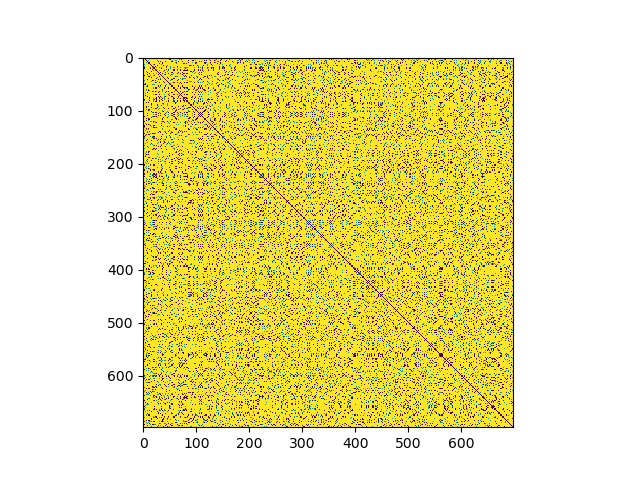
\includegraphics[width=.99\textwidth]{similarity_matrix.png}
\end{tcolorbox}
 
\item[(b)] (20 points) Implement the ISOMAP algorithm yourself to obtain a $k = 2$-dimensional embedding. This means, each picture is represented by a two-dimensional vector ($Z$ in the lecture), which we called ``embedding'' of pictures. Plot the embeddings using a scatter plot, similar to the plots in lecture slides. Find a few images in the embedding space and show what these images look like. Comment on do you see any visual similarity among them and their arrangement, similar to what you seen in the paper?
\begin{tcolorbox}
\textbf{Solution:} Firstly, pictures visually similar to each other are close in the scatter plot. Secondly, the arrangement of the pictures reflected a natural change of pattern. From pictures in the left to pictures in the right, the person gradually turned his face around from one side to the other side. From pictures on the bottom to pictures on the top, the person gradually turned his head from looking down to looking up. However, this scatter plot is not exactly the same as the one in the paper. The paper did a better job at distinguish the pictures on the top of my scatter plot.\\
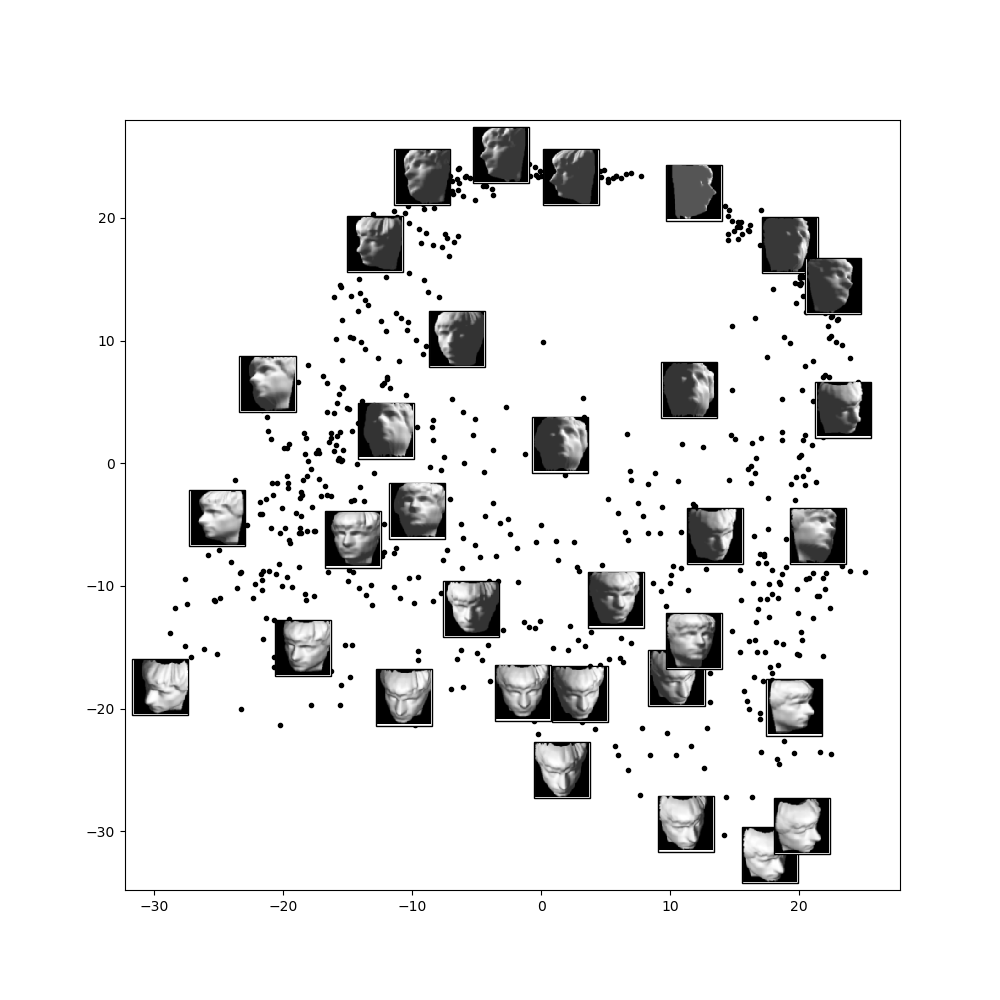
\includegraphics[width=.91\textwidth]{isomap_face_scatter.png}
\end{tcolorbox}

\item[(c)] (10 points) Now choose $\ell_1$ distance (or Manhattan distance) between images (recall the definition from ``Clustering'' lecture)). Repeat the steps above. Use $\epsilon$-ISOMAP to obtain a $k=2$ dimensional embedding. Present a plot of this embedding. Do you see any difference by choosing a different similarity measure by comparing results in Part (b) and Part (c)? 
\begin{tcolorbox}
\textbf{Solution:} Firstly, the components of the embedding using $l_1$ distance are much bigger than those using $l_2$ distance. Secondly, the points are more scattered with $l_1$ norm. Thirdly, the relative distance of pictures can also be different now. For example, the two pictures framed in red are close to each other under $l_1$ distance but far away from each other in $l_2$ distance. Personally, I think $l_2$ distance did a better job on these two pictures since the two gestures are very different.\\
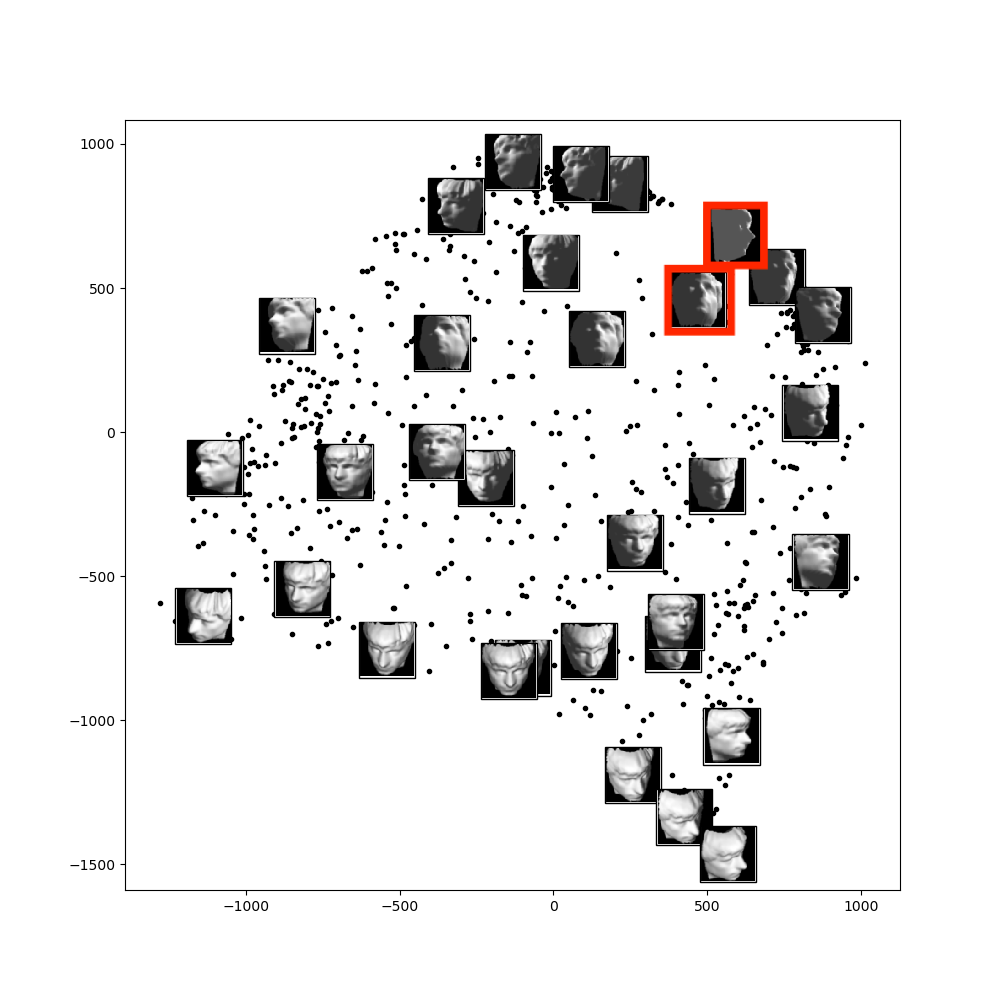
\includegraphics[width=1.0\textwidth]{face_scatter_l1.png}
\end{tcolorbox}
\newpage
\item[(d)] (10 points) Perform PCA (you can now use your implementation written in Question 1) on the images and project them into the top 2 principal components. Again show them on a scatter plot. Explain whether or you see a more meaningful projection using ISOMAP than PCA. 
\begin{tcolorbox}
\textbf{Solution:} Apparently, the ISOMAP algorithm provided a more meaningful projection. In the circled area of the following scatter plot from PCA, faces facing left and faces facing right are very close to each other. This means that PCA is not able to reflect the geodesic distance between pictures on a manifold.\\
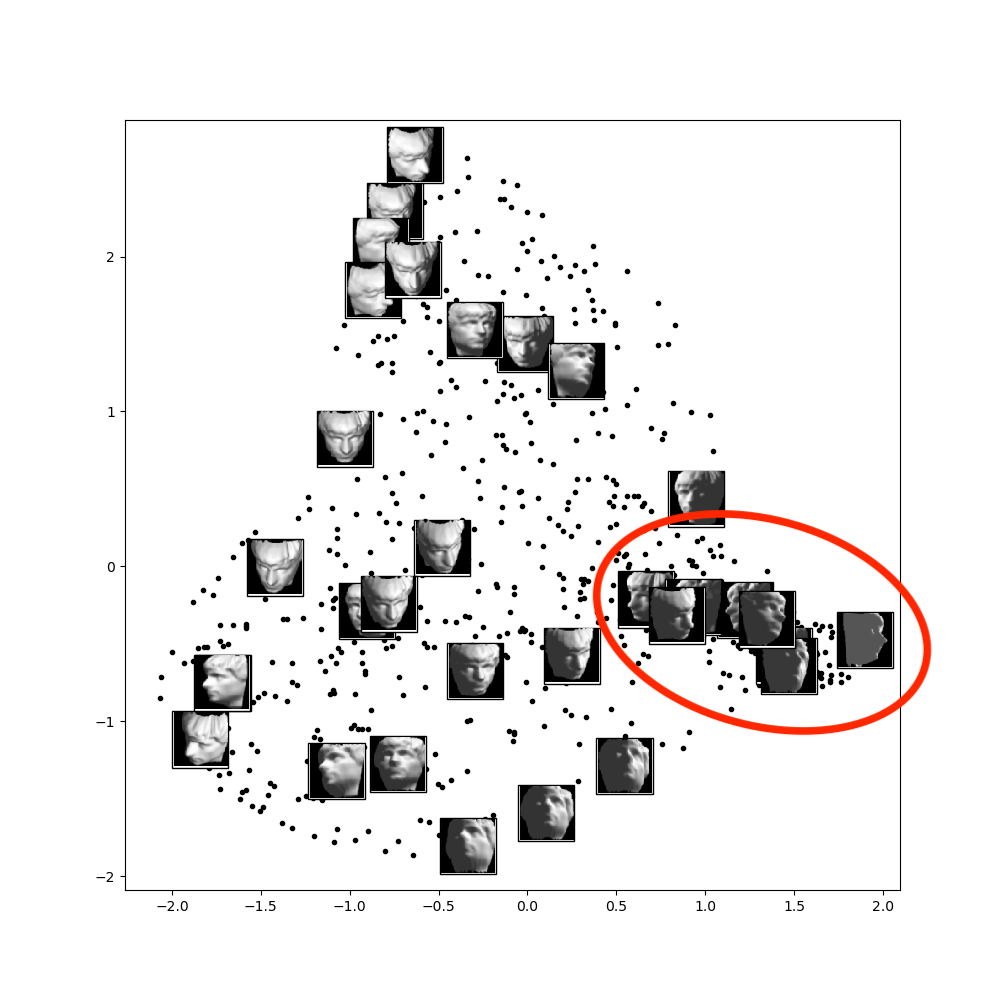
\includegraphics[width=.99\textwidth]{face_scatter_PCA.png}
\end{tcolorbox}

\end{enumerate}

\newpage

\subsection*{3. (Bonus) Eigenfaces and simple face recognition [15 points]}

This question is a simplified illustration of using PCA for face recognition. We will use a subset of data from the famous Yale Face dataset. {\bf Remark:} You will have to perform downsampling of the image by a factor of 4 to turn them into a lower resolution image as a preprocessing (e.g., reduce a picture of size 16-by-16 to 4-by-4). In this question, you can implement your own code or call packages. 

First, given a set of images for each person, we generate the eigenface using these images. You will treat one picture from the same person as one data point for that person. Note that you will first vectorize each image, which was originally a matrix. Thus, the data matrix (for each person) is a matrix; each row is a vectorized picture. You will find weight vectors to combine the pictures to extract different ``eigenfaces'' that correspond to that person's pictures' first few principal components. 


\begin{enumerate}

\item (10 points) Perform analysis on the Yale face dataset for Subject 1 and Subject 2, respectively, using all the images EXCEPT for the two pictures named \textsf{subject01-test.gif} and \textsf{subject02-test.gif}. {\bf Plot the first 6 eigenfaces for each subject.} When visualizing, please reshape the eigenvectors into proper images. Please explain can you see any patterns in the top 6 eigenfaces?
\begin{tcolorbox}
\textbf{Solution:} It seems like some of the eigenfaces are very similar to original faces, but some are not. For example, for Subject 1, the first two eigenfaces correspond to rightlight and leftlight, but it is hard to tell which face the third eigenface corresponds to.\\
\center{Eigenface for Subject 1}
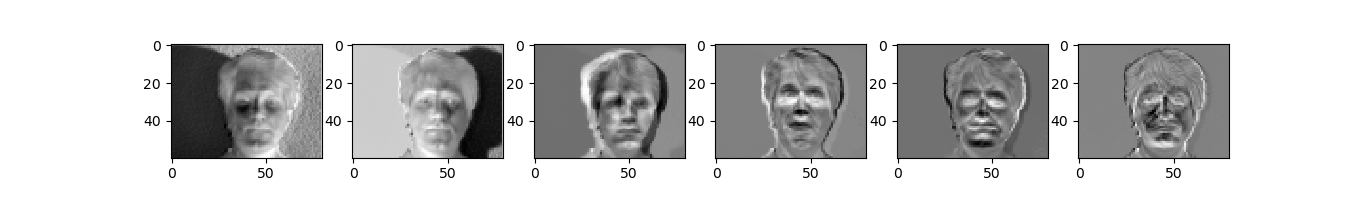
\includegraphics[width=1.0\textwidth]{eigenface1.png}
\center{Eigenface for Subject 2}
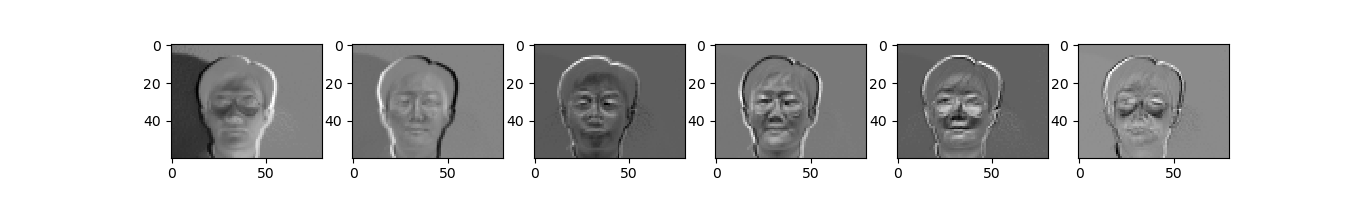
\includegraphics[width=1.0\textwidth]{eigenface2.png}
\end{tcolorbox}

\item (5 points) Now we will perform a simple face recognition task. 

Face recognition through PCA is proceeded as follows. Given the test image \textsf{subject01-test.gif} and \textsf{subject02-test.gif}, first downsize by a factor of 4 (as before), and vectorize each image. Take the top eigenfaces of Subject 1 and Subject 2, respectively. Then we calculate the {\it normalized inner product score} of the 2 vectorized test images with the vectorized eigenfaces:
\[s_{ij} =\frac{\textsf{(eigenface})_i^T \textsf{(test image)}_j}{\|\textsf{(eigenface}_i)\| \cdot\|\textsf{(test image)}_j\|}\]

Report all four scores: $s_{ij}$, $i = 1, 2$, $j = 1, 2.$ Explain how to recognize the faces of the test images using these scores. Explain if face recognition can work well and discuss how we can improve it, possibly. 
\begin{tcolorbox}
\textbf{Solution:} $s_{11} = -0.875$, $s_{21} = -0.555$, $s_{12} = -0.797$, $s_{22} = -0.628$. To recognize the faces of the test image $j$, we compare the absolute values of scores $s_{1j}$ and $s_{2j}$. If $|s_{1j}| > |s_{2j}|$, we recognize it as from the first subject. Otherwise, it belongs to the second subject. However, from our result we see only the first test face was recognized correctly. To improve it, I tried to use more than one eigenface to calculate the similarity scores and the difference between $s_{12}$ and $s_{2,2}$ became much smaller. However, $s_{12}$ is still a little bit larger than $s_{22}$. 
\end{tcolorbox}

\end{enumerate}


\end{document}
